% !TEX program = xelatex
\documentclass[usenames,dvipsnames]{beamer}
\usefonttheme{serif}
\usefonttheme{structuresmallcapsserif}
\usetheme{Warsaw}
% \usecolortheme{crane}
% Customize block colors based on the chosen theme
% \setbeamercolor{block title}{fg=red,bg=yellow} % Replace with actual color names
% \setbeamercolor{block body}{bg=white} % Replace with actual color nametitle.bg!10!bg}
\usepackage{xcolor}
\beamertemplatenavigationsymbolsempty
\usepackage{tikz}
\usepackage{pgfplots}
\renewcommand{\qed}{\hfill\blacksquare}
\newcommand{\D}[1]{\Delta #1}
\renewcommand{\a}{\alpha}
\usepackage{float}
% ============================================================ %
% HEBREW support via polyglossia %
% ============================================================ %
\usepackage{polyglossia}
\defaultfontfeatures{Mapping=tex-text, Scale=MatchLowercase}
\setdefaultlanguage{hebrew}
\setotherlanguage{english}
\newfontfamily\hebrewfont[Script=Hebrew]{Arial}
% Use \begin{hebrew} block of text \end{hebrew} for paragraphs.
% Use \texthebrew{ } and \textenglish{ } for short texts.
% ============================================================ %
\title[{}]{{מאקרו א' - $IS-LM$}}
\author{\texthebrew{ מתן לבינטוב}}
\institute[{ אב"ג}]{{ אוניברסיטת בן גוריון בנגב}}
\date{}

\usepackage{bidi}

\begin{document}
	\begin{RTL}
		\begin{frame}
			\titlepage
		\end{frame}

        % \section{הנחות מודל $IS-LM$}
        \begin{frame}
            \frametitle{ הנחות מודל  $ IS-LM $  }
            \begin{block}{הנחות}
                \begin{itemize}
                    \item התוצר נקבע בטווח קצר לפי ביקוש
                    \item בטווח קצר המחירים קשיחים
                    \item המשק יכול בנקודת שיווי משקל אשר גבוהה יותר או נמוכה יותר מתוצר פוטנציאלי
                \end{itemize}
            \end{block}
        \end{frame}


        \begin{frame}
            \frametitle{עקומת $IS$ - שוק המוצרים}
            עקומת $IS$ הינה העקומה אשר על גביה נמצאים אוסף הצירופים של תוצר וריבית אשר מביעים לש''מ בשוק המוצרים
            \begin{block}{נוסחאות}
                \begin{align*}
                    \begin{split}
                        IS : Y &= C + I + G \\
                        C & = C_0 + cY^d = C_0  + c\left( Y-T \ \right) \   ; \quad T = T_0 + tY \\
                        I & =   I_0 - bi \\ 
                        G &= G_0 \\ 
                    \end{split}
                \end{align*}
                \begin{equation*}
                    IS : Y = \alpha \left( A_0 - bi \right) \qquad \alpha = \frac{1}{1-c(1-t)} \: \text{המכפיל הקיינסיאני}
                \end{equation*}
                \begin{equation*}
                    A_0 = C_0 - cT_o + I_0 + G_0
                \end{equation*}
            \end{block}


        
        \end{frame}


        \begin{frame}
            \frametitle{שיפוע עקומת $IS$}
            \begin{block}{שיפוע עקומת $IS$}
                בגלל הצירים שיפוע העקומה צריך להיות לפי $\frac{\partial i}{\partial Y}$.
אולם יותר קל לגזור את העקומה שהיא לפי $\frac{\partial Y}{\partial i}$ ופשוט לעלות בחזקת מינוס 1
\begin{equation*}
    \frac{\partial Y}{\partial i} = - \alpha b \implies \frac{\partial i}{\partial Y } = \frac{-1}{\alpha b}
 \end{equation*}
            \end{block}
            
        
        \end{frame}

        \begin{frame}
            \frametitle{היסטים $IS$}
            \begin{alertblock}{$\D{IS}$}
                $\Delta Y = \alpha \left[\Delta A_0 - b\Delta i\right]$  
            \end{alertblock}
            
            \begin{block}{ היסט אופקי $\Delta i = 0 $}
                $\D{Y} = \a \D{A_0}$
            \end{block}

            \begin{block}{ היסט אנכי $\Delta Y = 0 $}
                $\D{i} = \dfrac{\D{A_0}}{b}$
            \end{block}

            
        
        \end{frame}
        \end{RTL}
        \begin{frame}
            \frametitle{עקומת $IS$}
            \begin{flushleft}
                \begin{tikzpicture}[scale=1.4]
                    \draw[->] (0,0) -- (6,0) node[right] {$Y$};
                    \draw[->] (0,0) -- (0,5) node[above] {$i$};
                    % \draw[dashed] (0,4) -- (4,0) node[midway, above left] {up} node[midway, below right] {down};
                    \draw [blue] (0.5,3.5) -- (4.5,0.5) node[midway, above left] {};
                    \node[right] at (3,3) {היצע עודף};
                    \node[left] at (2.5,1) {ביקוש עודף};
                    \node[right] at (4.5,0.5) {$IS$};
                \end{tikzpicture}
            \end{flushleft}
        
            
        
        \end{frame}


        \begin{RTL}
        
            
        \begin{frame}
            \frametitle{שוק הכסף $LM$}
            עקומת LM היא עקומה אשר על גביה נמצאים אוסף הצירופים של תוצר וריבית אשר מביאים לשיווי משקל
בשוק הכסף. 
\begin{block}{נוסחאות}
    \begin{align*}
        \begin{split}
           LM : \left(\frac{M}{P}\right) ^ d  & = \frac{M ^ s}{P} \\ 
           \left(\frac{M}{P}  \right) ^ d    & = \frac{M_0}{P} + kY - hi 
        \end{split}
    \end{align*}
    \begin{equation*}
        LM : i  = \frac{1}{h} \left[ky + \frac{M_0 - M^s}{P} \right]
    \end{equation*}
\end{block}

\begin{itemize}
    \item $M_0$ הינו מינע הביטחון
    \item $k$ מניע עסקאות
    \item $h$ מניע ספקולטיבי
\end{itemize}
        
            
        
        \end{frame}

        \begin{frame}
            \frametitle{עקומת $LM$}
            \begin{flushleft}
            \begin{tikzpicture}[scale=1.4]
                \draw[->] (0,0) -- (6,0) node[right] {$Y$};
                \draw[->] (0,0) -- (0,5) node[above] {$i$};
                % \draw[dashed] (0,4) -- (4,0) node[midway, above left] {up} node[midway, below right] {down};
                \draw [red] (0.5,0.5) -- (4.5,4.5) node[midway, above left] {};
                \node[right] at (1,3) {היצע עודף};
                \node[left] at (4,1) {ביקוש עודף};
                \node[right] at (4.5,4.5) {$LM$};
            \end{tikzpicture}
        \end{flushleft}
            
            
        
        \end{frame}

        \begin{frame}
            \frametitle{היסטים $LM$}
            \begin{alertblock}{$\D{LM}$}
                $\Delta i = \dfrac{1}{h} \left[k\D{Y} + \D{\frac{M_0}{P}} - \D{\frac{M^s}{P}}\right]$  
            \end{alertblock}
            
            \begin{block}{ היסט אופקי $\Delta i = 0 $}
                $\D{Y} = \dfrac{\D{\frac{M^s}{P}} - \D{\frac{M_0}{P}}}{k}$
            \end{block}

            \begin{block}{ היסט אנכי $\Delta Y = 0 $}
                $\D{i} = \dfrac{\D{\frac{M_0}{P}} - \D{\frac{M^s}{P}} }{h}$
            \end{block}

%             $\Delta i = \dfrac{1}{h} \left[k\D{Y} + \D{M_0} - \D{M^s}\right]$  \vspace{10pt}
% \\
% \textbf{היסט אופקי } $\Delta i = 0 $ \vspace{10pt} 
% \\
% $\D{Y} = \dfrac{\D{M^s} - \D{M_0}}{k}$ \vspace{10pt}
% \\ 
% \textbf{היסט אנכי } $\D{Y} = 0 $ \vspace{10pt}
% \\
% $\D{i} = \dfrac{\D{M_0} - \D{M^s} }{h}$
            
        
        \end{frame}
        \begin{frame}
            \frametitle{ש''מ כללי}
            קיים שילוב יחיד של תוצר וריבית אשר מביא לשיווי משקל בשוק המוצרים ובשוק הכסף במקביל לכל מצב
עולם.
שילוב של שתי העקומות הצבה של שוק הכסף בשוק המוצרים דרך הריבית.
\begin{block}{$IS-LM$}
    \begin{equation*}
        Y=\frac{\alpha h}{h+\alpha b k} \times A_0+\frac{\alpha b}{h+\alpha b k} \times\left(\frac{M^s-M_0}{P}\right)
    \end{equation*}
\end{block}
        
            
        
        \end{frame}

        \begin{frame}[allowframebreaks]
            \frametitle{גרפים}
        
            \begin{figure}[H]
                % \begin{small}
                    \begin{center}
                        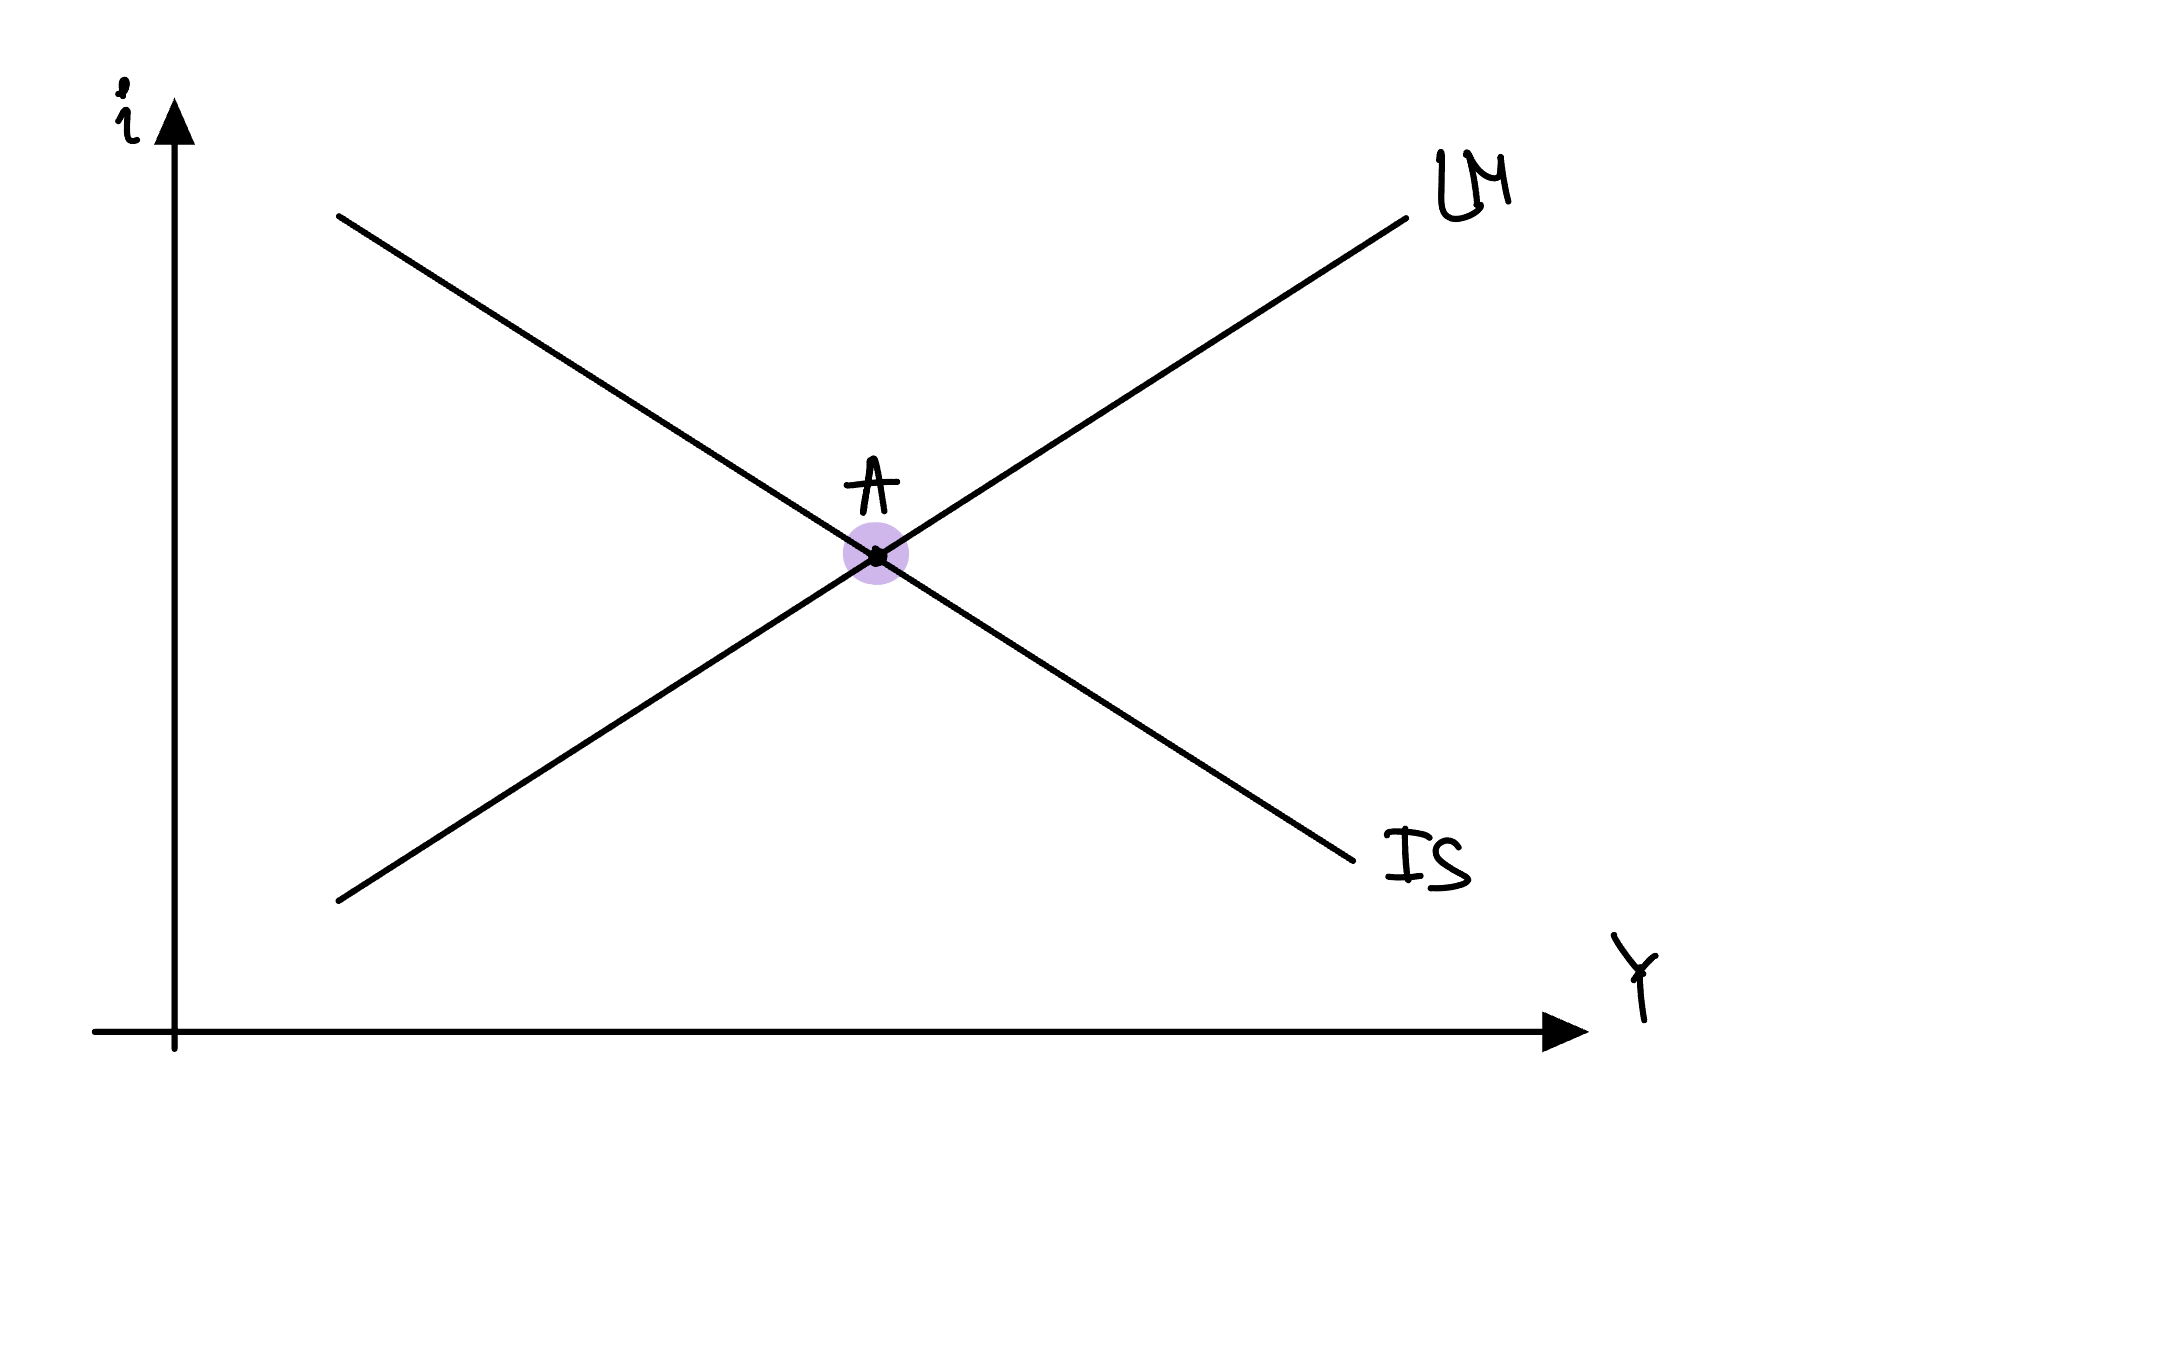
\includegraphics[width=0.95\textwidth]{figures/ISLM default.png}
                    \end{center}
                    % \caption{}
                    \label{fig:}
                % \end{small}
            \end{figure}
            
            \begin{figure}[H]
                \begin{small}
                    \begin{center}
                        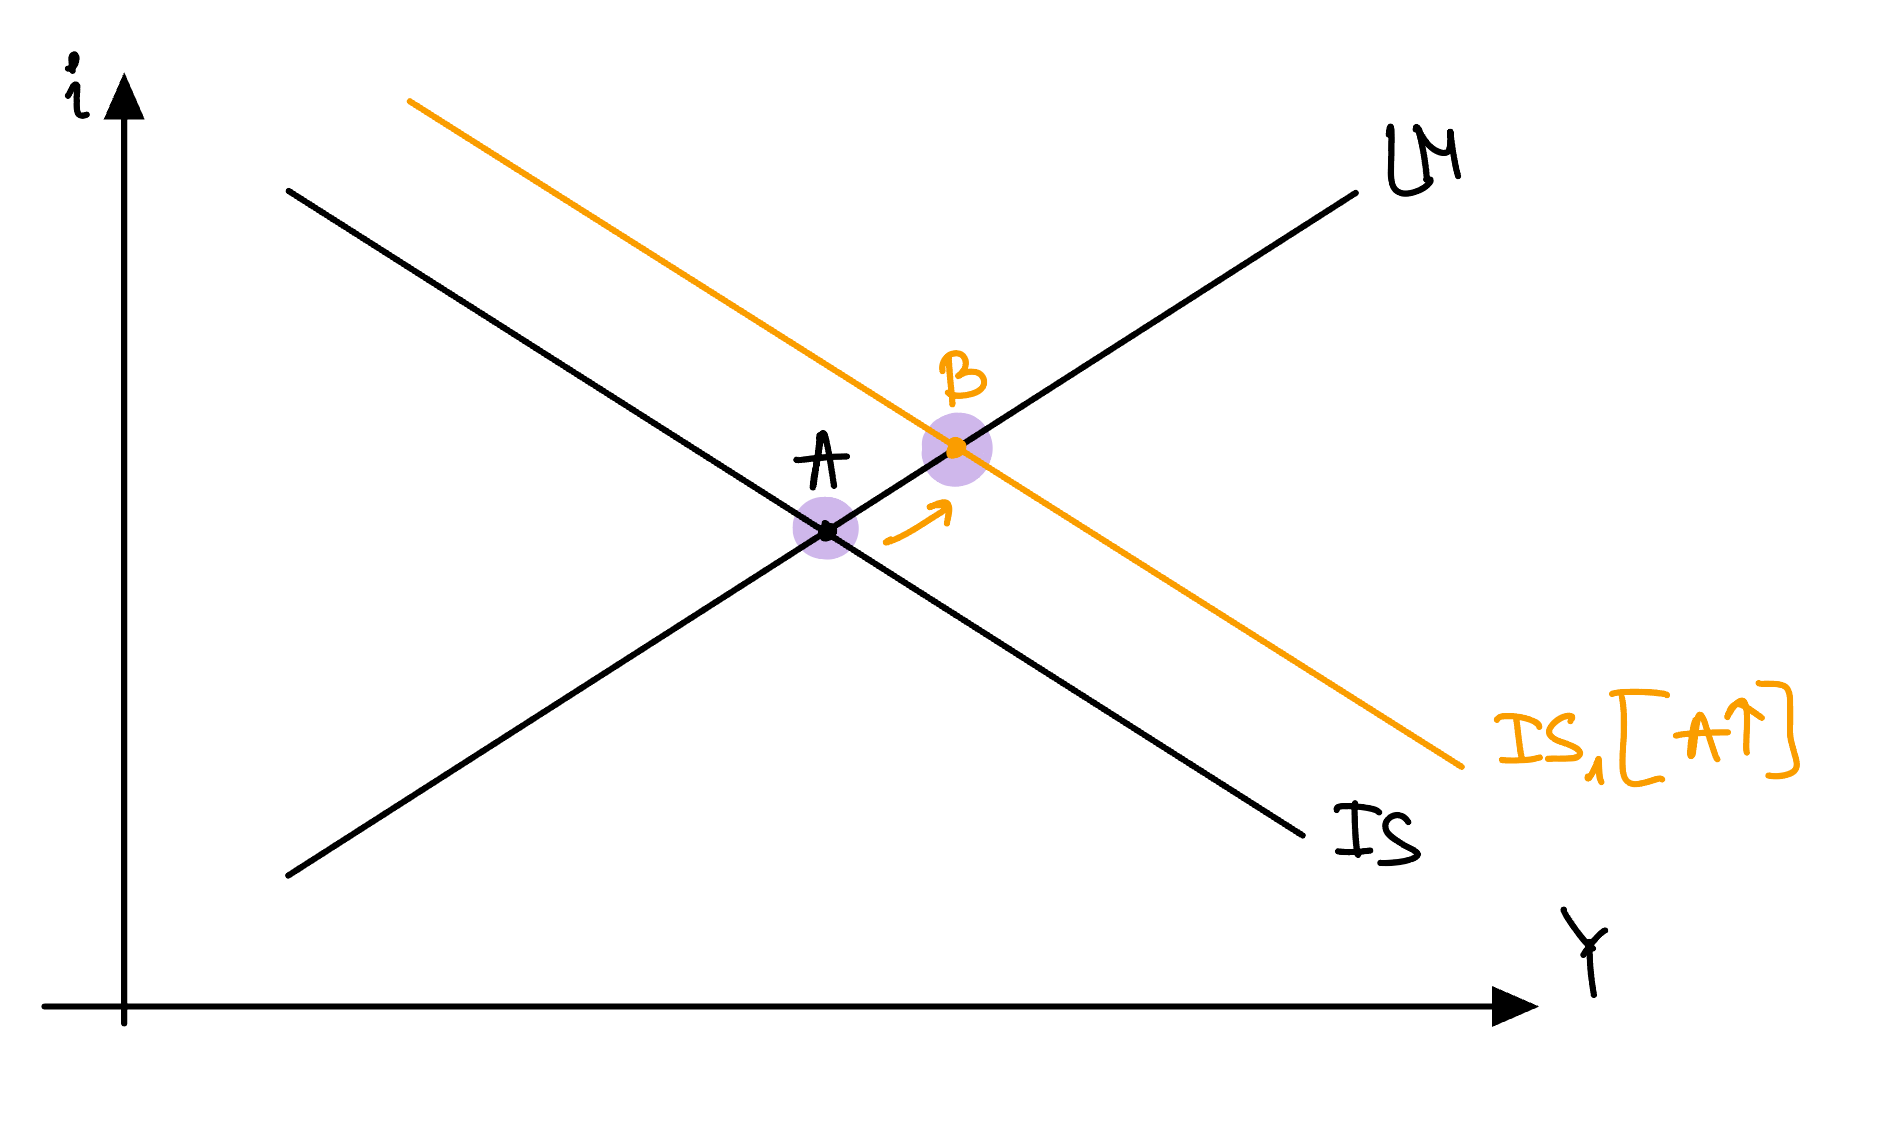
\includegraphics[width=0.95\textwidth]{figures/ISLM IS move.png}
                    \end{center}
                    % \caption{}
                    \label{fig:}
                \end{small}
            \end{figure}
            
            \begin{figure}[H]
                \begin{small}
                    \begin{center}
                        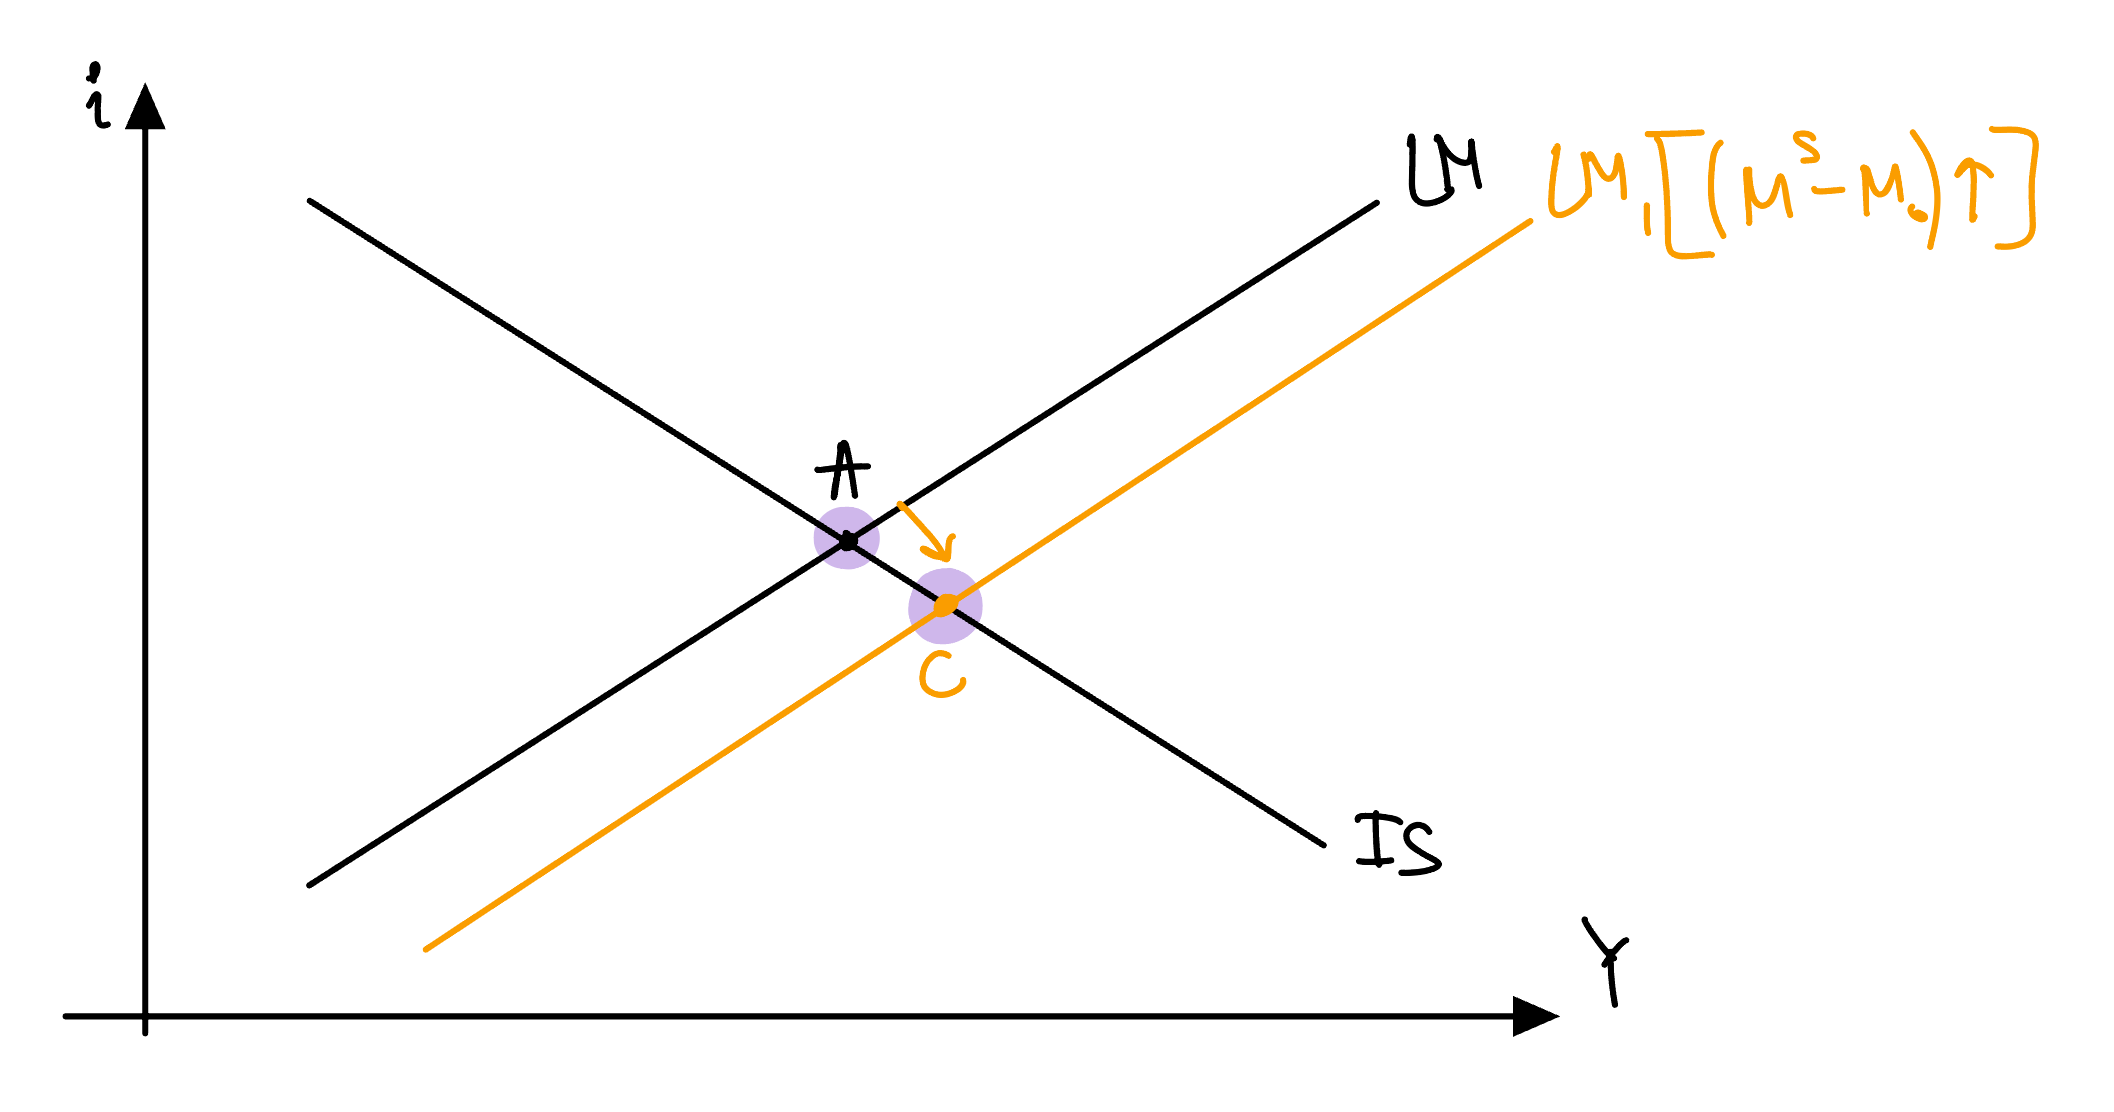
\includegraphics[width=0.95\textwidth]{figures/ISLM LM Move.png}
                    \end{center}
                    % \caption{}
                    \label{fig:}
                \end{small}
            \end{figure}
        
        \end{frame}
\end{RTL}
\end{document}